\chapter{Electronics and Software}
One of the constraints set early on in this project was keeping the robot low budget. This meant that no proprietary algorithms or software could be used; everything had to be free and open source. Luckily, the internet has a wealth of different options that people have created and make open for others to use.
\section{Inspiration}
The first step of any electronics design is establishing the feasibility of the design goal. Various examples were found on the internet demonstrating similar projects and inspiration was drawn from them to incorporate into this project. For instance, in a video by the YouTube channel Core Electronics showcased face tracking camera using OpenCV and a Raspberry Pi, shown in Figure \ref{fig:core-electronics}. This seemed to be a good proof of concept and was important in establishing the feasibility of this project, especially in such a short time frame. The problem with this model is that it is nothing more than a proof of concept, rather than a full product. It has minimal electronic components and the mechanism is fairly simple. The pan servo moves the tilt servo completely, which accomplishes two degrees of freedom, but is simplistic and most importantly does not resemble a natural eye nor does it resemble the dynamics of my eye mechanism. Another thing to note is the speed and smoothness of the motion of the face tracking mechanism leaves much to be desired, which was an area focused on in this project.

\begin{figure}[h]
    \centering
    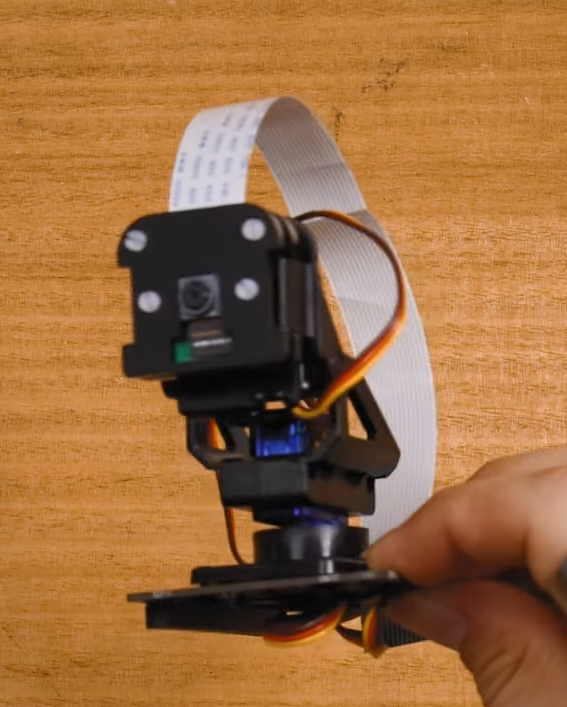
\includegraphics[width=0.3\linewidth]{Thesis/ch4/core-electronics.png}
    \caption{Pan and tilt mechanism used in the Core Electronics example.}
    \label{fig:core-electronics}
\end{figure}

\section{Components Selection}
\subsection{Microcontroller}
All components used in this project can be found in the Bill of Materials in Appendix \ref{ch:bom}. One important choice to note is the microcontroller, which is essentially the brain of the robot. The Teensy 4.0 was chosen for this for its low price but incredible speed. The Teensy can also be programmed in Arudino, which allows it to tap into the wealth of documentation and example code snippets online. To interface with the components it is possible to simply use a breadboard, but this project opted to leverage a dedicated robotics board to facilitate the process. This board, called PRT\_28 by Patton Robotics, provides numerous convenient features like a DC jack, voltage regulator, capacitors for despiking, and separate power rails for 12V and 5V. These are all components that could have been procured on their own, but for \$26 the board was the smarter choice given the time frame. A future version of the project would use a custom PCB that would allow for a large simplification of the circuitry. For instance, in hindsight much of the functionality of the Teensy is superfluous and can be accomplished with a much cheaper ATmega328P chip. Still, the Teensy accomplished what it was intended to, which was to serve as a way to control and synchronize the motion of the three motors in the robot.

\subsection{Actuators}
As stated in Section \ref{ch:design-iterations}, the motors chosen for the project were common, affordable parts. The servo model used in this design is the DS3218MG, with a control angle of $270^\circ$. 

Since the stepper motor is being geared up and the robot does not weigh much, the torque requirement on the stepper motor is not very large. As such, a smaller form factor was chosen to fit on the 8'' diameter base. The component chosen was a NEMA 14 stepper with 200 steps per rotation. With a control angle of 1.8 per step, these kinds of stepper motors are not known for their precision. However, this can be mitigated by gearing up the motor, which was explained previously, and choosing the right stepper motor driver.

To make the stepper motor spin, the electromagnetic coils in the motor have to be driven in the right order to spin the shaft. This can technically be done with the Teensy, but the smarter choice was to procure a daughter board with dedicated circuitry to efficiently drive the motor. This board, called the stepper driver, powers the stepper motor in accordance to signals from the Teensy. The one used in this project is a RepRap StepStick, running the A4988 chip \cite{bowyerStepStickRepRap2020}. This board communicates with the Teensy through two pins, denoted by the STEP and DIR (direction) pins. Every time the Teensy powers the STEP pin, the motor advances one step in the direction indicated by the state of the DIR pin. It is important to note that the motor is running at 12V, while the rest of the components use 5V. The stepper controller also serves the purpose of separating the two power lines and keeps the microcontroller safe from high voltage backflow. Another useful feature of the A4988 is microstepping, which allows the motor to move at fractions of a step. This enables much greater precision than the base 200 steps per revolution of the motor. For the greatest precision and smoothness of the movement, the lowest microstepping configuration was selected at 1/16 step, now giving the motor 3200 steps per revolution. Combined with the 1:6 gear ratio, this allows the stepper motor to rotate the robot with a resolution of $200\times16\times6=19200$ steps per revolution, or $0.01875^\circ$ per step.

\subsection{Miscellaneous}
A 12V 5A AC adapter of was used to deliver power to the circuit. The 12V of the jack powers the stepper motor directly and passes through a voltage regulator to power the rest of the 5V circuitry.

Additional components include a speaker and microphone which were incorporated into the design for a nominal user to have a natural conversation with the robot listening and responding. The current functionality is limited to playing sound files from a Python script, but the main purpose of including these components was to future proof the design for features that are planned to be included later down the line.

\section{Circuit Diagrams}
The circuit diagram used to wire up the components can be seen in Figure \ref{fig:circuit_diagram}. Note that the only components that had to be wired up were the Teensy microcontroller, the two servos, the stepper motor and its associated motor controller board. The other components, such as the camera, microphone, speaker, and the Teensy serial data cable all used a plain USB 2.0 connector, so they simply needed to be plugged into a USB hub and connected to the computer. One thing to note is that the 5V power line of the Teensy USB cable is cut. This isolates the Teensy power from the laptop and allows the laptop to communicate with the microcontroller over the two data lines without the potential of any backflow voltage that could damage the laptop. These USB cables come out of the back of the robot's head, pictured in Figure \ref{fig:back-wires}.

\begin{figure}[h]
    \centering
    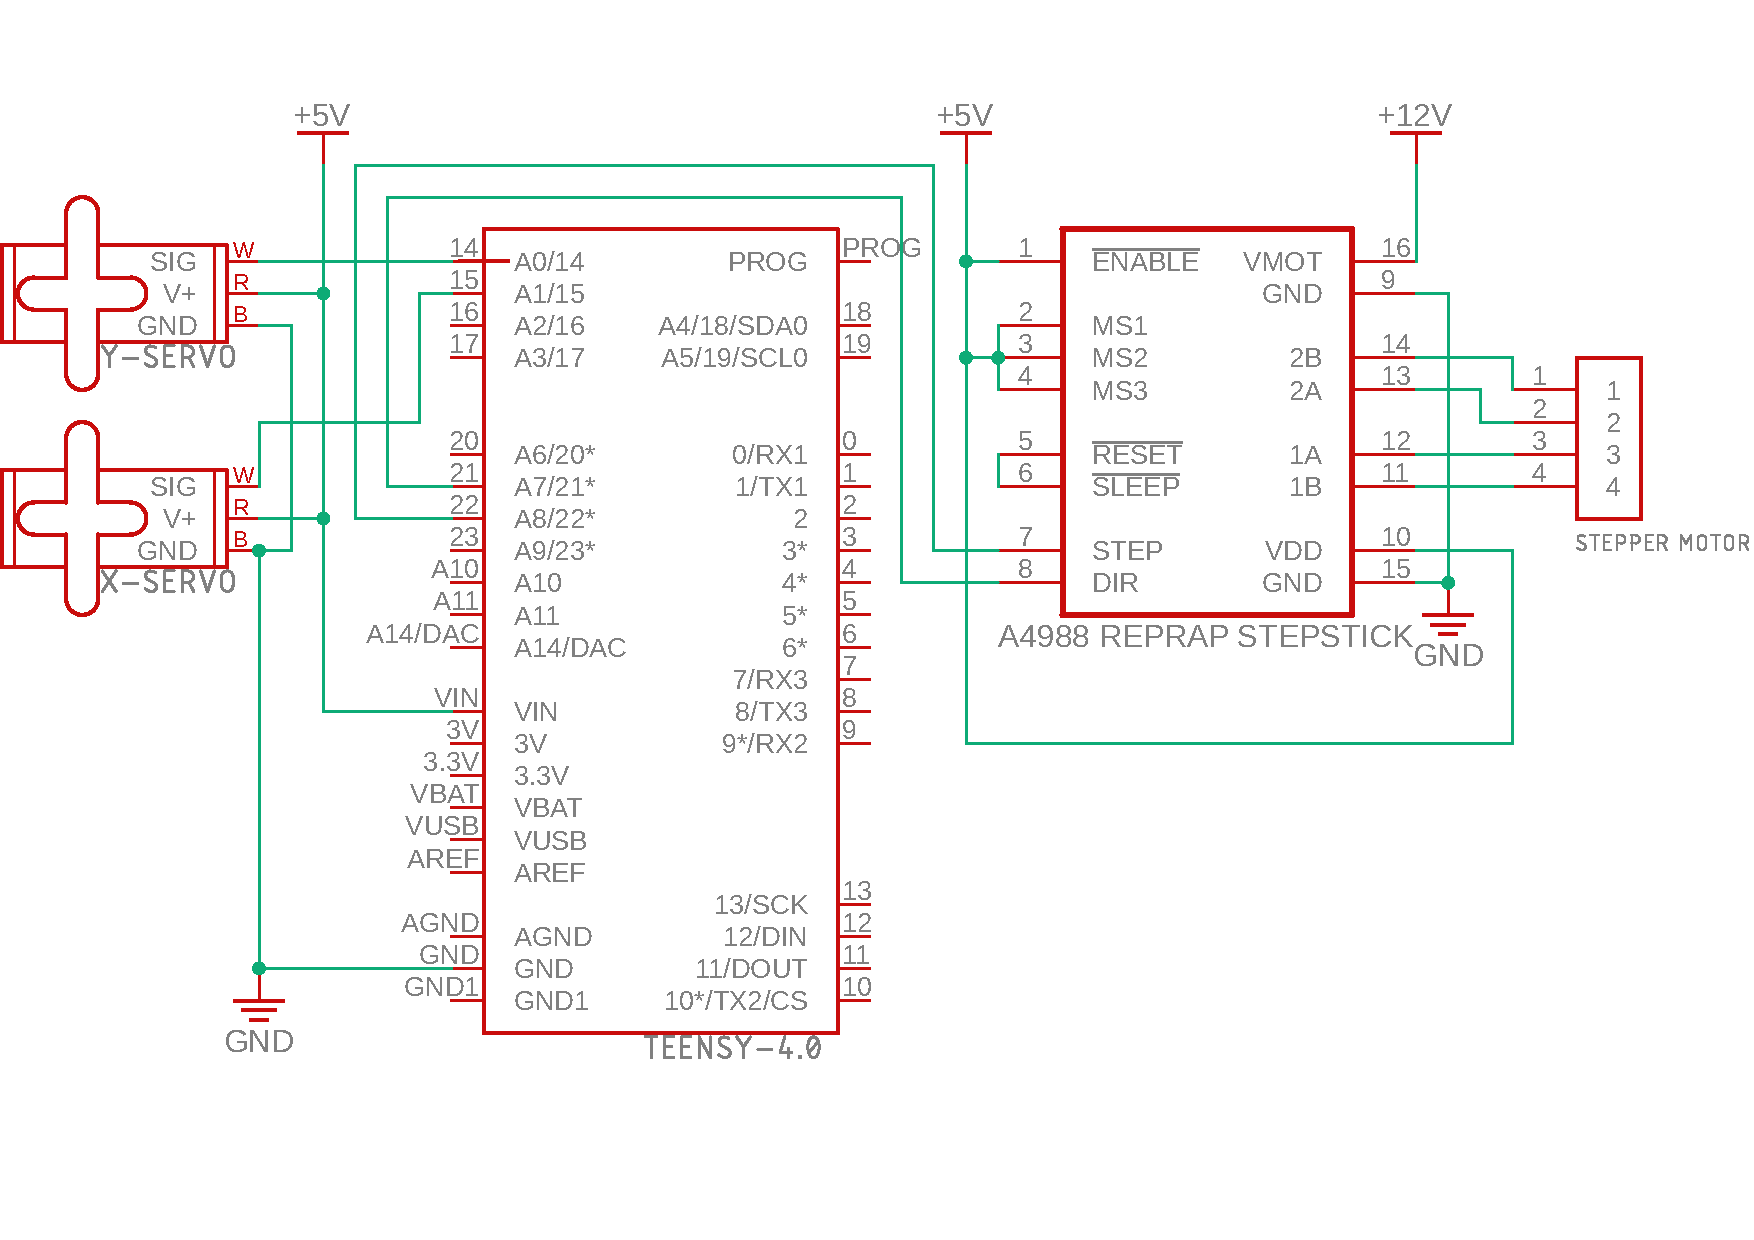
\includegraphics[width=0.8\linewidth]{Thesis/ch4/theses-schematic-2.pdf}
    \caption{Electrical schematic of the circuit. Generated in Autodesk EAGLE.}
    \label{fig:circuit_diagram}
\end{figure}

\begin{figure}[h]
    \centering
    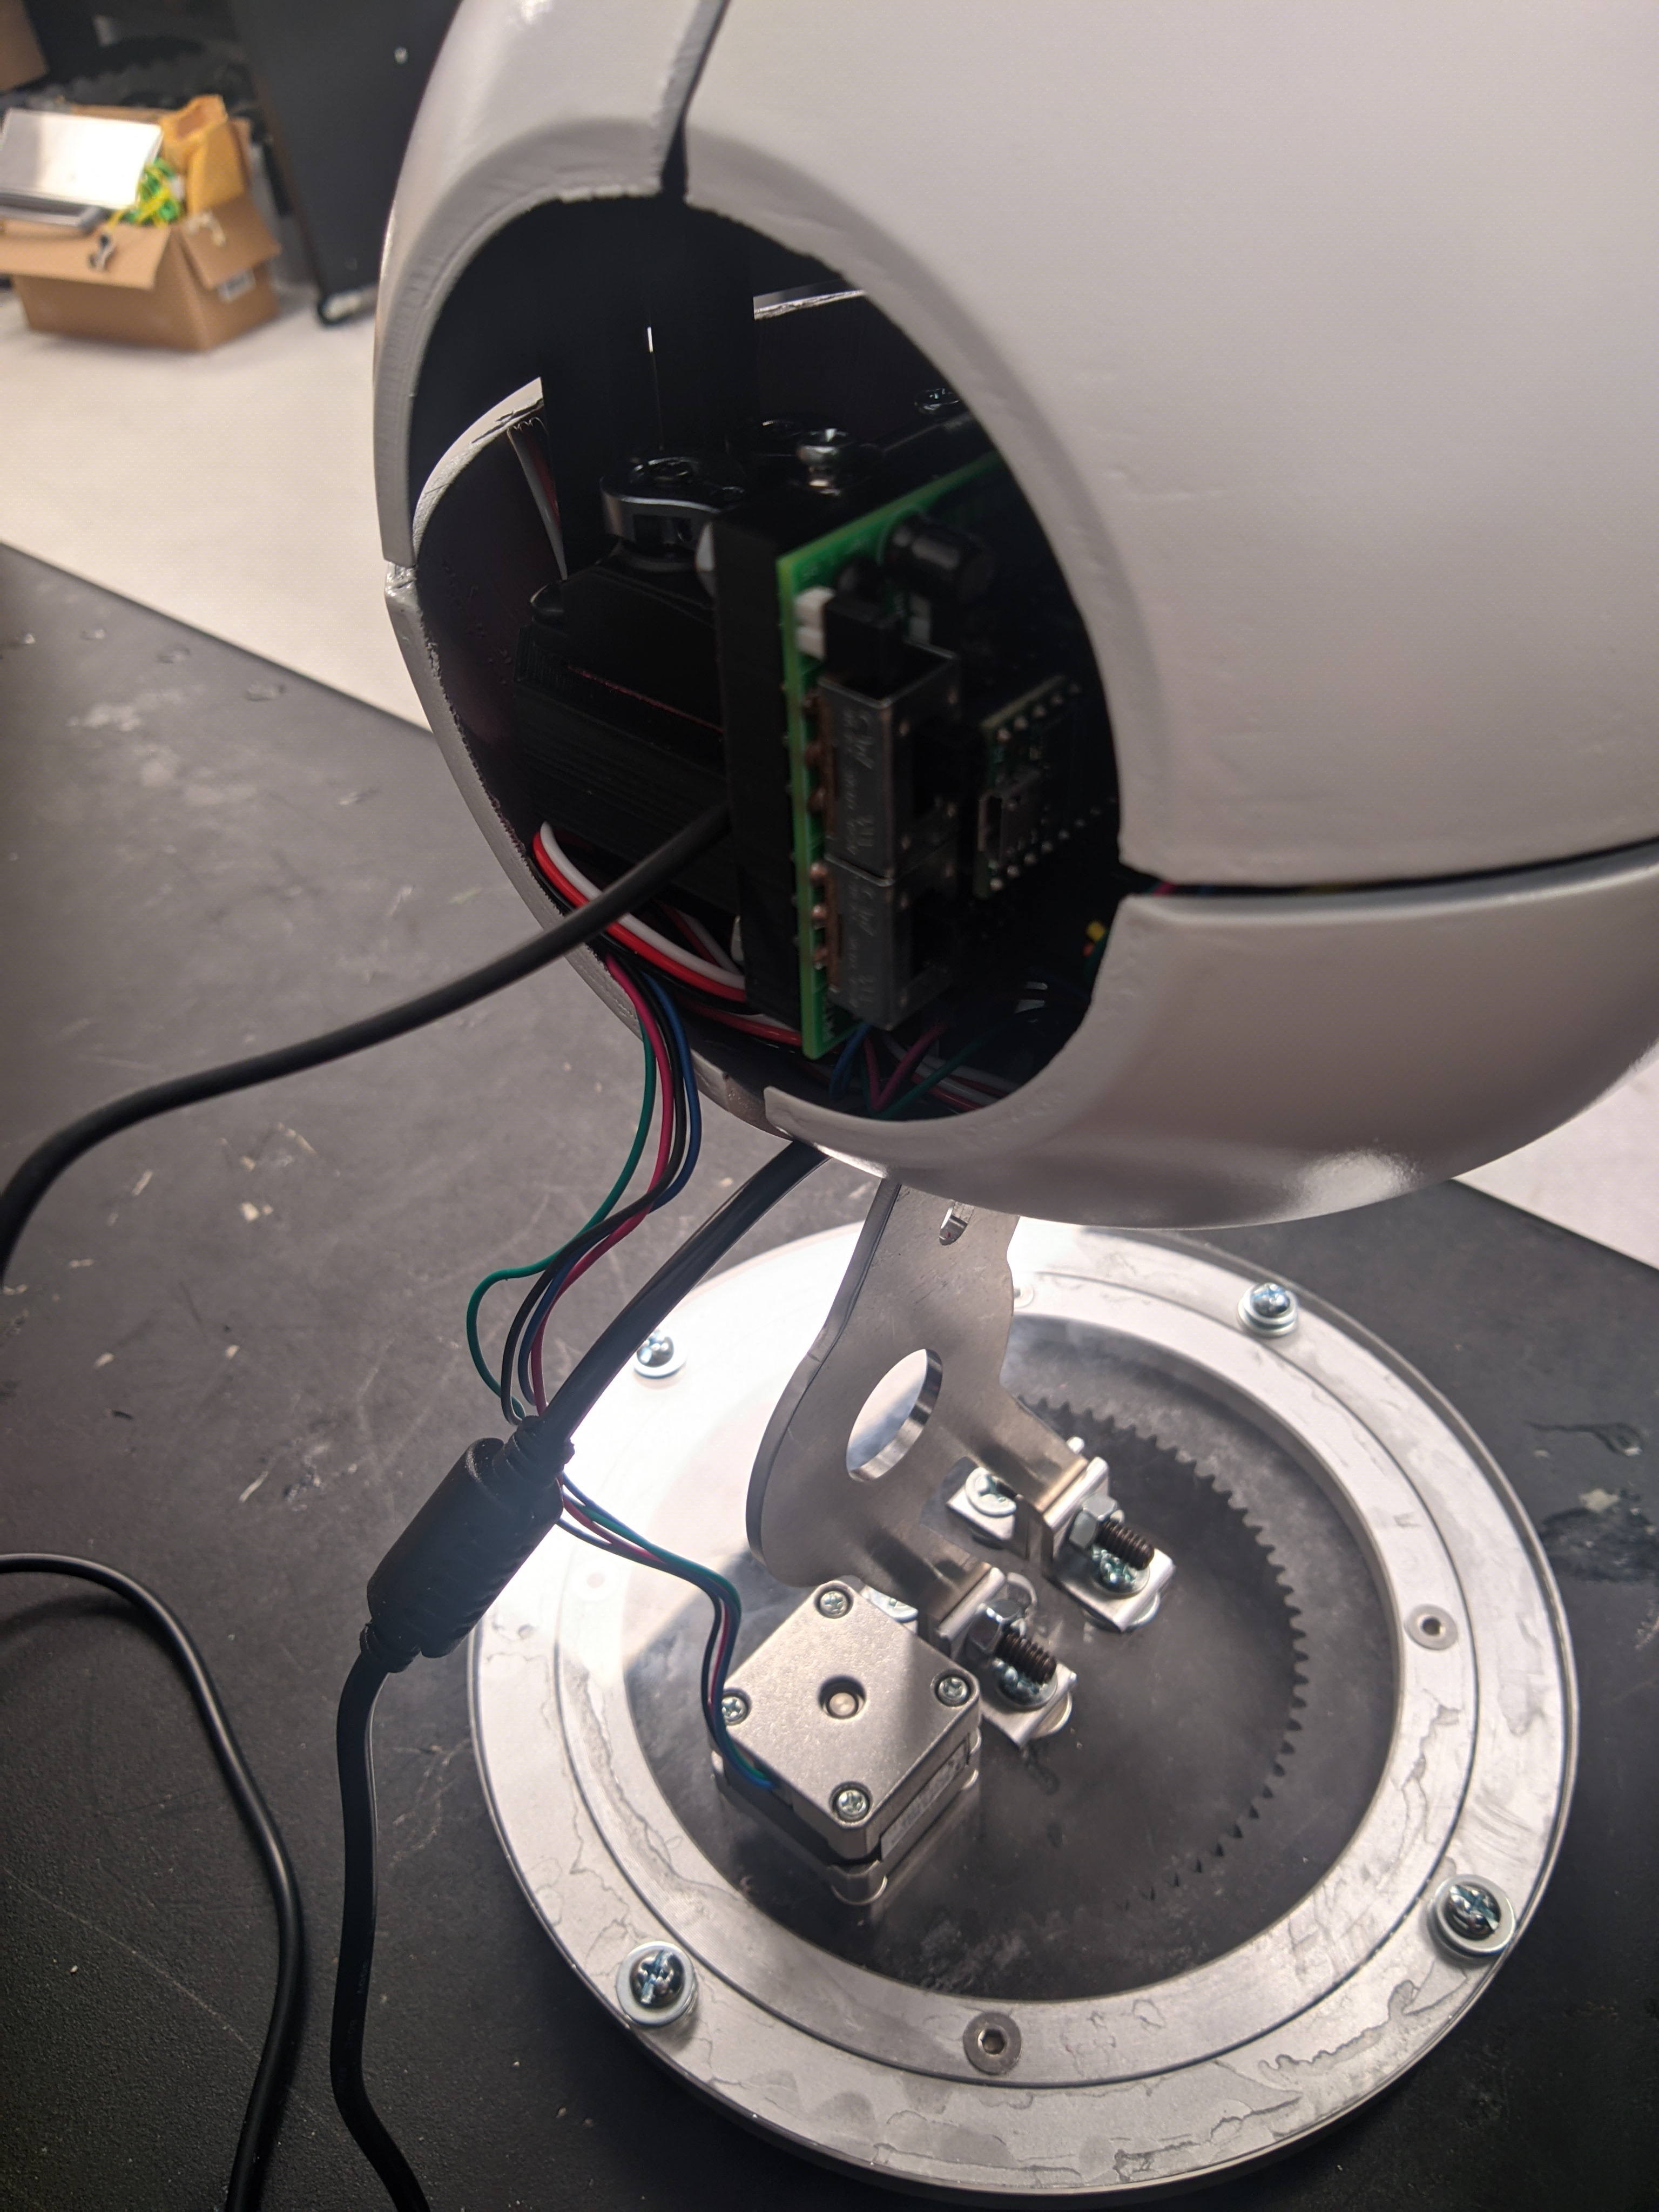
\includegraphics[width=0.4\linewidth]{Thesis/ch4/back-wires.jpg}
    \caption{A photo showing the wires coming out of the back of the head.}
    \label{fig:back-wires}
\end{figure}
\section{Software and Programming}
The algorithm for following the eyeball needed to be simple but also fast. One measure taken was avoiding the practice of blocking, which is when the processor waits for one action to finish before beginning the next. This would essentially freeze the Arduino when any motor is running and rather than all the motors moving at once, causing them to move one after the other. Instead, the code utilized software libraries that used non-blocking code to drive the actuators, which enabled all the components to move at the same time. This helps with smoothing out the motion of the system and keeping the robot more appealing to interact with. 

\subsection{Software Libraries Used}
\begin{itemize}
    \item Python
    \begin{itemize}
       \item OpenCV 2 \cite{OpencvOpencv2023}
        \item face\_recognition \cite{geitgeyFaceRecognition2023a}
        \item pySerialTransfer \cite{powerbroker2PySerialTransfer2023}
    \end{itemize}
    \item Arduino
    \begin{itemize}
        \item SerialTransfer \cite{pb2SerialTransfer2023}
        \item ServoEasing \cite{arminServoEasing2023}
        \item AccelStepper \cite{AccelStepperAccelStepperLibrary}
    \end{itemize}
\end{itemize}

\subsection{Control Loop}
Figure \ref{fig:control_loop} shows the control loop for the program. The control is discrete rather than analog, since the microcontroller runs in discrete time steps. The algorithm is as follows: First, the camera on the computer turns on and receives an image. An example of the image output from the camera is shown in Figure \ref{fig:face-example}. Then, the Python facial recognition library is used to find the center of the bounding box drawn around the face in the image and calculates the distance from that point to the center of the image. This distance is then scaled by a constant and sent as a move command to the motors. One effect of this approach is that larger move commands are sent to the motor as the face is farther from the center of the screen. This ensures that the camera will reach the face in fewer moves than a constant stepping distance. As the face gets closer to the center of the image, the motor commands are smaller, giving the system the ability to perform micro adjustments to center the camera properly.

A deadzone is used to decide whether or not to command the motors, since it is practically impossible that the face will be at the very center pixel of the image. The deadzone chosen for this was the middle 6\% of the width and height of the image. This seemed to provide a good balance between allowing for imperfect alignments while still producing a convincing face-tracking result to the user.

The servo and stepper motors in turn move the camera, which then captures a new image and the cycle repeats. It is important to note that the move commands are relative to the actuator's current position, so the Python code does not actually know what position the motors are at. All it sees is the camera footage and sends commands to the Teensy. Once the Teensy is ready to receive a command, it picks the most recent one out of the stack and executes it. Of course, there are some hard coded limits in the code to make sure the actuators do not exceed the maximum designed range of motion, which would cause the machine to tear itself apart, which is discussed in more detail in Section \ref{ch:safety}.

To decide when to use the stepper vs the X-servo to correct the x-position of the camera image, the X-servo was set to run 70\% of the distance total distance and the stepper was set to run 30\%, so that when they are run at the same time they center the camera correctly.

The control loop models a proportional controller, since the control output linearly scales with the measured input. The full Python and Arduino code can be found in Appendices \ref{ch:python-code} and \ref{ch:arduino-code}, respectively. Lots of the skeleton code for this algorithm was based on examples provided by face\_recognition, pySerialTransfer, and SerialTransfer.

\begin{figure}[h]
    \centering
    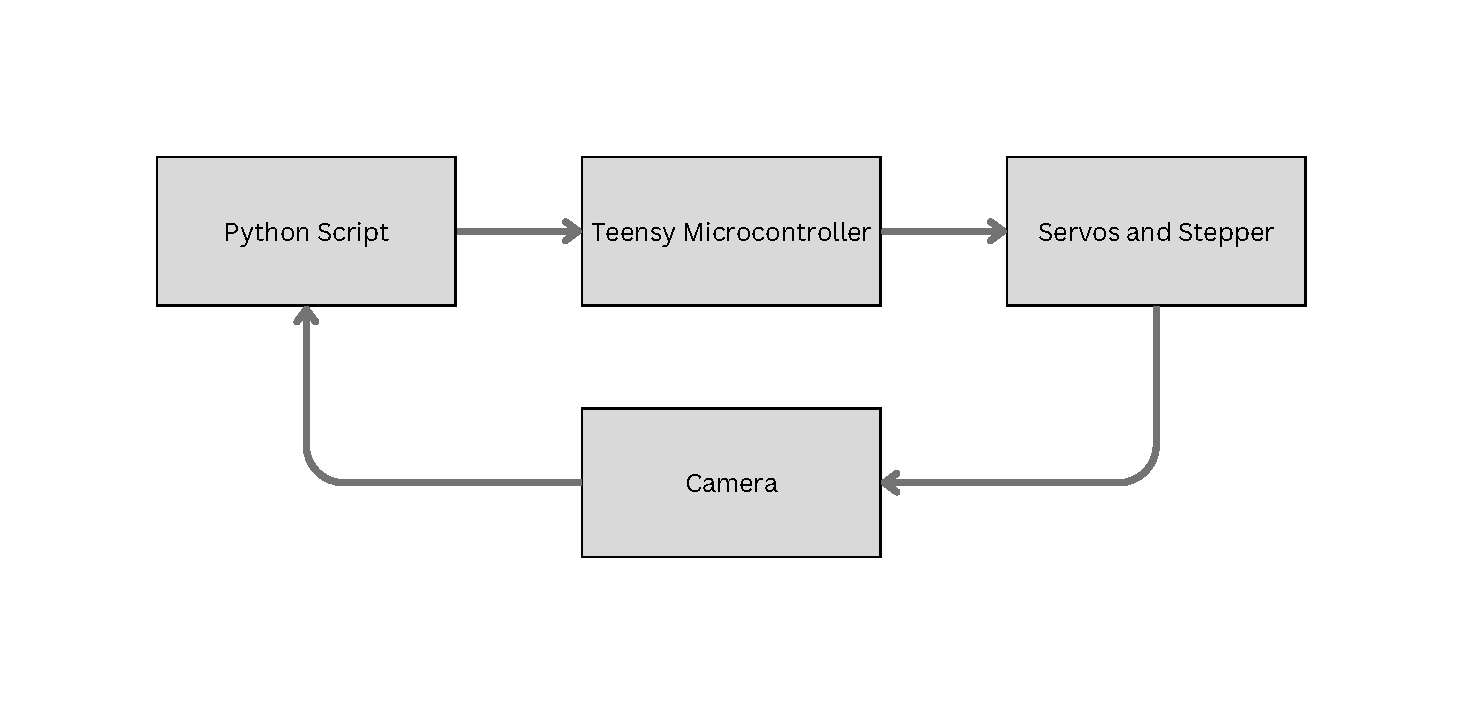
\includegraphics[width=0.9\linewidth]{Thesis/ch4/Microcontroller (3).pdf}
    \caption{Control Loop for the face tracking algorithm.}
    \label{fig:control_loop}
\end{figure}

\begin{figure}
    \centering
    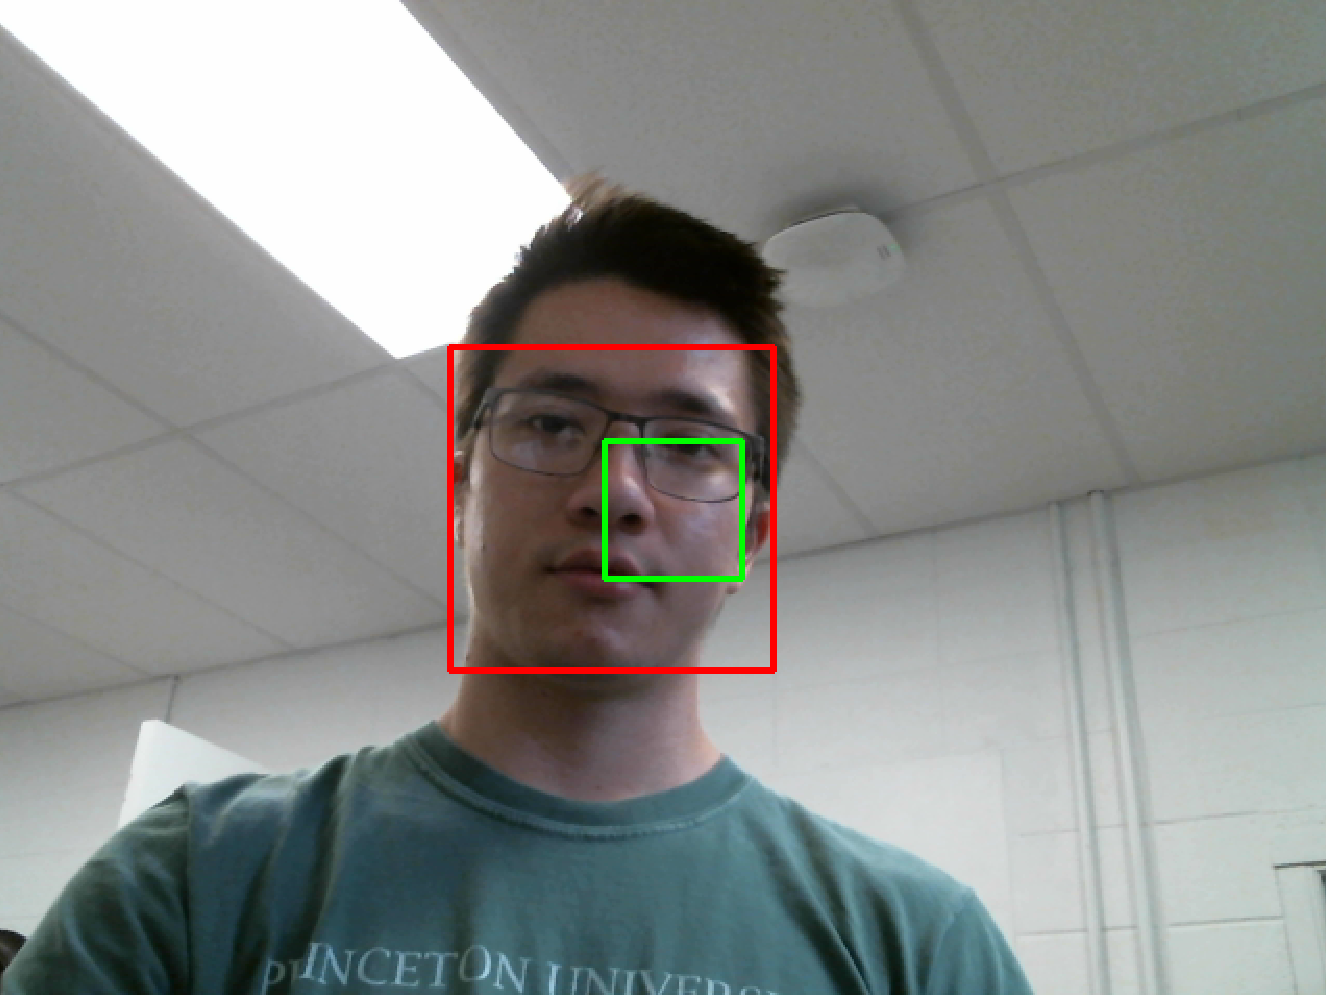
\includegraphics[width=0.5\linewidth]{Thesis/ch4/face-example.png}
    \caption{Example of what is displayed on the screen for facial recognition.}
    \label{fig:face-example}
\end{figure}

\section{Actuator Range of Motion}
\label{ch:safety}
To command the servos to move to a set position, the microcontroller sends it a PWM pulse in the range of 500-2500 ms, where 1500 ms is the middle position of the motor's range of motion. The eye mechanism does not need the full 270 degrees range of motion of the servos, in fact if the servos rotate that far it will tear the mechanism apart, which happened multiple times by accident. For this reason the millisecond ranges allowed to be sent to the servo were trimmed. 

The mechanism was designed so that the motors would hold the eye in a neutral position looking straight ahead when the servos are in their middle 1500 ms position. However, due to assembly imperfections this was not actually the case, so the motors had to be calibrated to find the servo position that would produce the desired neutral position of the eye. As such, after some experimentation these limits were empirically set to 1200-1670 ms for the Y-servo and 1320-1680 ms for the X-servo. Translating this into real world measurements, this means that the arm of the Y-Servo and X-Servo can sweep through an angle of $63.45^\circ$ and $48.6^\circ$, respectively. The stepper motor limits were determined such that the beyond $180^\circ$ in either direction to protect the cables from getting wrapped up. Since a full rotation of the robot would be 19200 steps, the limits on the motor were set to 9560 steps in either direction.

A confusing detail to note is that in the software the ends of the servo rotation are called 0 and 180, but these are just arbitrary variables. The true angular displacement of the robot is scaled according to the inputted ``angle'' and the microsecond range previously mentioned. For instance, a servo command of 90 to both motors resets the mechanism and returns it to the neutral looking ahead state. For simplicity, from this point forwards the servo angles will be referred to by their software variables rather than their real world counterparts.

\section{Integration}
Integrating these different components together was a significant challenge. Most notably, the facial recognition library is written in Python and is too computationally intensive to be run on a microcontroller, so the code has to be run on a PC instead. The PC then has to communicate with the Teensy through the Python script to tell the microcontroller how it should move the actuators. Fortunately, the serial data system is designed for this purpose.

Serial data allows for digital data to be sent through electrical signals in a cable to the microcontroller. This data can then be interpreted as a integer, character, or other any data type. This works both ways as well, so the microcontroller can also send values to the PC. This is a relatively trivial task if only one value is being sent to the Teensy, since Arduino has built in serial libraries for this purpose. For instance, I can type in the letter b on my computer and the PC sends it over the USB cable, then the microcontroller can recognize that data and do something with it, like printing out the value or moving a servo according to an inputted number. \cite{ansh2919SerialCommunicationPython2021}\cite{detheFaceTrackingOpenCV2019}. However, the challenge is controlling multiple actuators at once. The stock Arduino library uses blocking code, so this would slow down the system tremendously. Also, the microcontroller needs some way to identify which commands to send to which motor. This can be done with the base Arduino library \cite{robin2SerialInputBasics2016}, but a more complete solution was to use pySerialTransfer.

The pySerialTransfer library takes advantage of the C data structure \emph{struct}, which allows for packaging multiple variables into a single data structure. This struct is composed of the two servo move commands and the stepper move command. This allows us to separate the move commands into distinct variables that can be read and used by the microcontroller. The struct is first filled with values by the Python script based on the previously mentioned methodology, then the Python script fills a buffer with the struct. Once it finishes putting all three values in the buffer, it sends it off to the Teensy with serial data. The library pySerialTransfer interprets this serial data and fills in the corresponding struct in the Arduino script with the appropriate move commands. Then, the Teensy can use these values to actuate the motors accordingly. The full setup, including the robot and laptop, can be seen in Figure \ref{fig:complete-setup}.

\begin{figure}[h]
    \centering
    \includegraphics[width=0.5\linewidth]{Thesis/ch4/full-setup.jpg}
    \caption{Photo of the entire setup.}
    \label{fig:complete-setup}
\end{figure}